\chapter{Охрана труда и окружающей среды}
\section{Анализ условий труда}
\subsection{Обеспечение условий труда в отделе разработки программного обеспечения}
Дипломная работа посвящена разработке системы мониторинга состояния ЛА на основе алгоритмов интеллектуального анализа данных. Разработка производится на персональном компьютере и предполагает длительное пребывание за ним инженера.

Применение персонального компьютера освобождает человека от непроизводительной работы, связанной с обработкой информации, изменяет характер его труда. Однако при этом увеличивается доля умственного и нервно-напряженного труда, возрастает психоэмоциональная нагрузка. При значительной трудовой нагрузке, нерациональной организации работы и неблагоприятных факторах производственной среды быстро снижается работоспособность операторов, уменьшается производительность труда и ухудшается качество работы, может развиться перенапряжение,~а в отдельных случаях возникнуть срыв трудовой деятельности~--- дистресс.

В данном разделе проводится анализ условий труда в отделе разработки информационных систем с целью обеспечения безопасности и удобства, требуемых для работы инженера.

\subsection{Характеристика помещения}
Помещение находится в здании Московского Авиационного Института и представляет собой кафедральную лабораторию со следующими размерами:
\begin{itemize}
	\item длина~6~м;
	\item ширина~4~м;
	\item высота~3.5~м.
\end{itemize}

Площадь: $6\times4 = 24$~м\textsuperscript{2}.

Объём: $6\times4\times3,5 = 84$~м\textsuperscript{3}.

Количество рабочих мест~---~4.

Количество одновременно находящихся в помещении сотрудников не превышает~4 человек.

План помещения приведён на рисунке~\ref{fig:labourprotection:room_plan}.
\begin{figure}[h]
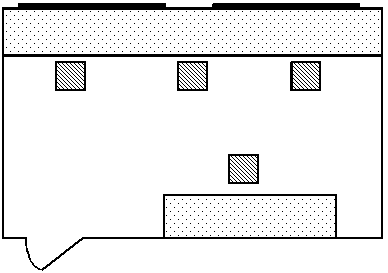
\includegraphics[width=0.6\textwidth, keepaspectratio]{plan}
\caption{План помещения}\label{fig:labourprotection:room_plan}
\end{figure}

Нормативные требования к площади и объёму рабочих мест определены в \cite{SanPin2_2_2}:
\begin{itemize}
	\item площадь на одно рабочее место с ВДТ или ПЭВМ для взрослых пользователей должна составлять не~менее~6~м\textsuperscript{2};
	\item объём~---~не~менее~20~м\textsuperscript{3}.
\end{itemize}

Фактические значения на каждого сотрудника:
\begin{itemize}
	\item площадь: $24/4 = 6$~м\textsuperscript{2};
	\item объём: $84/4 = 21$~м\textsuperscript{3}.
\end{itemize}

Данные значения показывают, что кафедральная лаборатория полностью соответствует установленным нормам.

В помещении имеются 2 оконных проёма высотой 1,6~м и шириной 2,3~м, которые выходят на юго-запад.

Искусственное освещение представляет собой 6~светильников, расположенных параллельно окнам в~2~ряда.

\subsection{Характеристика производственного процесса}
Разработка программного обеспечения производится на ПЭВМ с подключенными к ней периферийными устройствами.

\subsection{Характеристика используемого оборудования}
В процессе разработки используется следующее оборудование:
\begin{enumerate}
	\item{ПЭВМ:}
		\begin{enumerate}
			\item{процессор Intel Core i5 3,60 ГГц;}
			\item{оперативная память 8 Гб;}
			\item{жёсткий диск 1 Tб;}
			\item{напряжение питания 220 В.}
		\end{enumerate}
	\item{ЖК монитор с диагональю 23 дюйма (58,42) ASUS VX239H:}
		\begin{enumerate}
			\item{частота 75 Гц;}
			\item{яркость 250 кд/м\textsuperscript{2};}
			\item{динамическая контрастность 8 000 000 : 1;}
			\item{напряжение питания 220 В.}
		\end{enumerate}
	\item{Клавиатура Logitech K330;}
	\item{Мышь A7Tech X;}
	\item{Принтер HP LaserJet 1005M:}
		\begin{enumerate}
			\item{напряжение питания 220 В.}
		\end{enumerate}
\end{enumerate}

\subsection{Санитарно-гигиенические факторы}

\subsubsection{Микроклимат помещения}
Микроклимат в рабочем помещении должен соответствовать \cite{GOST12_1_005}.

Согласно \cite{GOST12_1_005}, работа разработчика ПО относится к категории «Легкая~–~Iа», т.к. лёгкие физические работы~--- работы с расходом энергии не более 150 ккал (174 Вт), а категория Iа подразумевает энергозатраты до 120~ккал/ч~(139 Вт).

Рабочее место разработчика ПО является постоянным, т.к. он находится на нём большую часть рабочего времени (более~50\%).

Нормативные и фактические значения для категории работ «Легкая~–~Iа», лёгкие физические работы~--–~работы с расходом энергии не более 150~ккал (174~Вт). Категория Iа подразумевает энергозатраты до 120~ккал/ч (139~Вт).

Рабочее место разработчика модели является постоянным, т.к. он находится на нём большую часть рабочего времени (более 50\%).

Нормативные и фактические значения для категории работ «Легкая – Iа» и постоянного рабочего места приведены в таблице~\ref{tab:labourprotection:microclimat}.

\begin{table}[h]
\caption{Значения характеристик микроклимата помещения}
\label{tab:labourprotection:microclimat}
\nohyphenation

\begin{tabular}{|C{84pt}|C{178.25pt}|C{101.1pt}|C{110pt}|}
\hline
 & Температура, \textdegree C & Относительная влажность, \% & Скорость движения, м/с \\
\hline
Допустимые значения & 22--24~–-- Холодный период \linebreak 23--25~--– Теплый период & 40--60 & 0.1 \\
\hline
Фактические значения & 22--24~–-- Холодный период \linebreak 25--30~--– Теплый период & 45--55 & <0.1 \\
\hline
\end{tabular}
\end{table}

Фактические значения параметров микроклимата данного помещения удовлетворяют допустимым значениям для холодного периода года. Во время теплого периода в помещении может преобладать повышенная температура из-за отсутствия кондиционера, который бы мог её регулировать.

\subsubsection{Производственное освещение}
Освещённость регламентируется~\cite{SNiP23_05_95}.

Наименьший размер объекта различения в работе инженера составляет 0.3 мм. Объектом является символ, выводимый на экран монитора (наименьшим символом является точка). Зрительная работа относится к III разряду --- высокая точность (наименьший размер объекта различения от 0.3 до 0.5~мм).

Контраст объекта с фоном средний, фон светлый, что соответствует подразряду~б разряда III.

Требования к освещению помещений промышленных предприятий для подразряда~б разряда III:
\begin{itemize}
	\item При системе комбинированного освещения освещенность равна: всего --- 1000 лк, в т.ч. от общего --- 200 лк;
	\item При системе общего освещения освещённость равна 300 лк.
\end{itemize}

Система освещения в комнате общая, состоящая из 6 потолочных светильников ЛПО 46, в каждом из которых установлены 4 люминесцентные лампы ЛТБ мощностью 20 Вт и световым потоком 1100 лм. Светильники расположены в два ряда параллельно окнам. Фактическая освещенность составляет 275 лк, что полностью удовлетворяет нормативным значениям~\cite{SNiP23_05_95}.

\subsubsection{Шум}
Источники шума в данном помещении: охлаждающие системы ПЭВМ (охлаждение процессоров).

Уровни шума на рабочих местах инженера ПЭВМ должны соответствовать~\cite{GOST12_1_003}.

Допустимые значения уровня шума при проектировании и программировании на рабочих местах в помещениях – проектно-конструкторских бюро; расчётчиков, программистов вычислительных машин, в лабораториях для теоретических работ и обработки данных: не более  50 дБА.

Фактические значения уровня шума: не более 45 дБА, что подтверждается расчётами в пункте~\ref{sec:labourprotection:calc}.

Согласно~\cite{GOST12_1_003}, значения уровня шума на рабочем месте удовлетворяют установленным требованиям.

\subsubsection{Электромагнитное излучение}
Во время работы ПЭВМ возникают электромагнитные поля, которые оказывают негативное влияние на организм человека.

Источниками электромагнитных полей на рабочем месте инженера являются системные блоки. Современные корпуса системных блоков ПЭВМ позволяют значительно ослабить излучения его элементов. Благодаря существующим достаточно строгим стандартам дозы рентгеновского излучения от современных мониторов и системных блоков не опасны для пользователей.

Документом, регламентирующим уровень электромагнитного излучения для ПЭВМ, является~\cite{SanPin2_2_2}.

Согласно ему, напряжённости электрических и магнитных полей, энергетической нагрузки в течение рабочего дня не должны превышать значений, указанных в таблице~\ref{tab:labourprotection:emradiation}.

\begin{table}[h]
\caption{Предельные значения электромагнитного излучения.}
\label{tab:labourprotection:emradiation}
\nohyphenation

\begin{tabular}{|C{213.35pt}|C{87.35pt}|C{84.4pt}|C{83.4pt}|}
\hline
\multirow{2}{\hsize}{\centering{Параметр}} & \multicolumn{3}{C{255.15pt}|}{Предельные значения в диапазонах частот, МГц} \\
\cline{2-4}
 & от 0.06 до 3 & св. 3 до 30 & св. 30 до 300 \\
\hline
Е\textsubscript*{ПД}, В/м & 500 & 300 & 80 \\
\hline
Н\textsubscript*{ПД}, А/м & 50 & --- & --- \\
\hline
ЭН\textsubscript*{Е\textsubscript*{ПД}}, (В/м)\textsuperscript{2} $\cdot$ ч & 20000 & 7000 & 800 \\
\hline
ЭН\textsubscript*{Н\textsubscript*{ПД}}, (А/м)\textsuperscript{2} $\cdot$ ч & 200 & --- & --- \\
\hline
\end{tabular}
\end{table}

Монитор ASUS VX239H соответствует стандарту~\cite{TCO03}, который устанавливает следующие предельные значения электромагнитного излучения:
\begin{itemize}
	\item напряжённость электрического поля: в диапазоне 5Гц--2кГц не более 10~В/м, в диапазоне 2кГц--400кГц не более 1.0~В/м;
	\item напряжённость магнитного поля: в диапазоне 5Гц--2кГц не более 200~нТл, в диапазоне 2кГц--400кГц не более 25~нТл.
\end{itemize}

Данные характеристики полностью соответствуют требованиям~\cite{SanPin2_2_2}.

\subsection{Электроопасность}
В данном помещении используется оборудование, питающееся от сети переменного тока напряжением 220~В, частотой 50~Гц. 

Согласно~\cite{PUE7}, помещение отдела разработки ИС относится к классу помещений без повышенной опасности поражения электрическим током: это сухое помещение с непроводящими полами, с нормальной температурой воздуха и влажностью, в нем отсутствует токопроводящая пыль.

Электрооборудование в помещении представлено мониторами и системными блоками ПЭВМ. Источником электрического поражения может быть металлический корпус системного блока при пробое изоляции, т.к. имеется напряжение 220~В, а в~\cite{GOST12_1_038} допустимое напряжение и ток для аварийных режимов при времени воздействия более 1~секунды составляют 20~В и 6~мА.

\subsection{Пожароопасность}
В данном помещении имеются твердые горючие и  трудногорючие веще-ства и материалы (книги, документы, деревянная мебель, оргтехника и т.д.), которые при взаимодействии с огнем будут гореть без взрыва. Также источником возгорания может быть электрическая проводка.

Согласно~\cite{GOST12_1_004}, данное помещение относится к классу Б и является пожароопасным.